\documentclass[11pt,a4paper]{article}
\usepackage[margin=2.3cm]{geometry}
\usepackage{amsmath,amssymb}
\usepackage{booktabs,tabularx,array}
\usepackage{tikz}
\usepackage{xcolor}
\usepackage[hidelinks]{hyperref}
\usepackage{enumitem}
\setlist{itemsep=2pt,topsep=4pt}
\setlength{\parskip}{4pt}
\setlength{\parindent}{0pt}

\newcommand{\Hz}{H_0^{(1)}}
\newcommand{\Ho}{H_1^{(1)}}
\newcommand{\inc}{\mathrm{inc}}

\title{Rough slab under beam illumination:\\ scoping the extension of the pysie2d boundary integral method}
\author{pysie2d design notes}
\date{24 September 2026 --- draft 1}

\begin{document}
\maketitle

\begin{abstract}
\noindent
This note works out what it takes to apply Maradudin's rough-surface method
(Maradudin \emph{et al.}, Ann.\ Phys.\ 203, 255, 1990) to a film: two rough,
flat-on-average surfaces extending to infinity, with a laterally bounded
Gaussian beam coming from above. Starting from the boundary conditions, it
derives the four coupled integral equations and shows that they have the same
building blocks as the pysie2d matrix: each surface contributes a copy of the
single-particle $2\times2$ block, and the two surfaces are coupled through the
slab. The one new difficulty is that truncating infinite surfaces fails once
roughness couples light into guided modes, which carry power sideways to the
cut ends. The flat slab has an exact closed-form answer, and it cannot excite
guided modes, so it is a clean first validation anchor. Rough-surface physics
also needs a small-roughness perturbation anchor.
\end{abstract}

%======================================================================
\section{Geometry, media and conventions}

\begin{center}
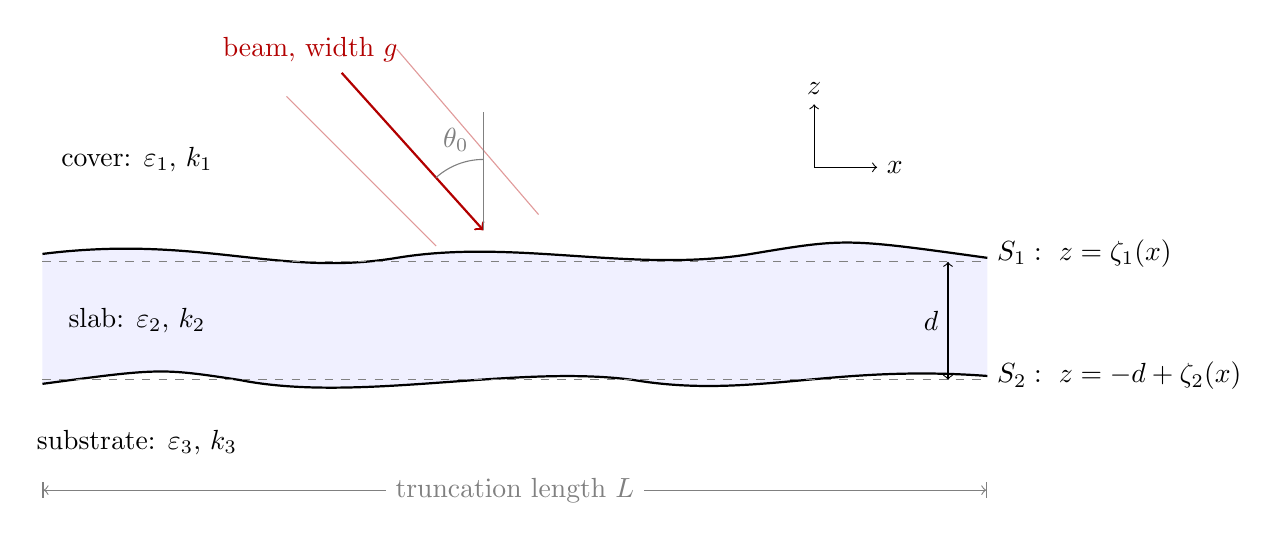
\begin{tikzpicture}[scale=1.0]
  \fill[blue!6] (-6,0.1) .. controls (-4,0.35) and (-3,-0.2) .. (-1.5,0.05)
     .. controls (0,0.3) and (1.5,-0.15) .. (3,0.1) .. controls (4.2,0.3) .. (6,0.05)
     -- (6,-1.45) .. controls (4,-1.3) and (3,-1.75) .. (1.5,-1.5)
     .. controls (0,-1.3) and (-2,-1.8) .. (-3.5,-1.5) .. controls (-4.5,-1.35) .. (-6,-1.55) -- cycle;
  \draw[thick] (-6,0.1) .. controls (-4,0.35) and (-3,-0.2) .. (-1.5,0.05)
     .. controls (0,0.3) and (1.5,-0.15) .. (3,0.1) .. controls (4.2,0.3) .. (6,0.05);
  \draw[thick] (-6,-1.55) .. controls (-4.5,-1.35) .. (-3.5,-1.5)
     .. controls (-2,-1.8) and (0,-1.3) .. (1.5,-1.5) .. controls (3,-1.75) and (4,-1.3) .. (6,-1.45);
  \draw[dashed,gray] (-6,0) -- (6,0);   \draw[dashed,gray] (-6,-1.5) -- (6,-1.5);
  \node[right] at (6,0.1) {$S_1:\ z=\zeta_1(x)$};
  \node[right] at (6,-1.45) {$S_2:\ z=-d+\zeta_2(x)$};
  \node at (-4.8,1.3) {cover: $\varepsilon_1$, $k_1$};
  \node at (-4.8,-0.75) {slab: $\varepsilon_2$, $k_2$};
  \node at (-4.8,-2.3) {substrate: $\varepsilon_3$, $k_3$};
  \draw[->,thick,red!70!black] (-2.2,2.4) -- (-0.4,0.4);
  \draw[red!70!black,opacity=.4] (-2.9,2.1) -- (-1.0,0.2);  \draw[red!70!black,opacity=.4] (-1.5,2.7) -- (0.3,0.6);
  \node[red!70!black] at (-2.6,2.7) {beam, width $g$};
  \draw[gray] (-0.4,0.4) -- (-0.4,1.9); \draw[gray] (-0.4,1.3) arc (90:132:0.9); \node[gray] at (-0.75,1.55) {$\theta_0$};
  \draw[<->] (5.5,0) -- (5.5,-1.5); \node[left] at (5.5,-0.75) {$d$};
  \draw[|<->|,gray] (-6,-2.9) -- (6,-2.9); \node[gray,fill=white] at (0,-2.9) {truncation length $L$};
  \draw[->] (3.8,1.2) -- (4.6,1.2) node[right] {$x$};  \draw[->] (3.8,1.2) -- (3.8,2.0) node[above] {$z$};
\end{tikzpicture}
\end{center}

Everything is invariant along $y$, so, as in pysie2d, a single scalar field
$\psi(x,z)$ describes each polarisation:
\begin{itemize}
  \item \texttt{pol = 2}, TE: $\psi = E_y$;
  \item \texttt{pol = 1}, TM: $\psi = H_y$.
\end{itemize}
The time dependence is $e^{-i\omega t}$ and lengths are in nm. Each medium $j$ has a
complex permittivity $\varepsilon_j$ and wavenumber
$k_j = \sqrt{\varepsilon_j}\,2\pi/\lambda_{\mathrm{vac}}$. In every medium the field satisfies
$\nabla^2\psi + k_j^2\psi = 0$, and the free-space Green function is the one
pysie2d already uses:
\begin{equation}
  G_j(r) = \tfrac{i}{4}\,\Hz(k_j r).
\end{equation}
Only the slab is allowed to be lossy. The cover and substrate must be lossless so
that far-field reflection and transmission exist (see \S6).

\paragraph{Surface unknowns.} As in Maradudin's paper, both surfaces are written as
height profiles, parametrised by $x$ and sampled over $-L/2<x<L/2$. On each surface there are two unknown functions:
\begin{itemize}
  \item $\phi_m(x)$: the field on surface $S_m$;
  \item $\chi_m(x)$: the derivative along the \emph{un-normalised} upward normal,
        $\chi = \left(-\zeta_m'\,\partial_x + \partial_z\right)\psi$.
\end{itemize}
Because $\chi$ carries the length element $ds = \sqrt{1+\zeta'^2}\,dx$, every surface integral below reduces to a plain $\int dx'$.
This is the same idea as pysie2d's $\chi$ carrying the Jacobian of $t$ (conventions \S5).
On $S_1$, $\chi_1$ is taken on the cover side; on $S_2$, $\chi_2$ is taken on the slab side.

%======================================================================
\section{Boundary conditions}

On each surface, the tangential $E$ and $H$ are continuous. For the scalar field this becomes:
\begin{equation}
  \psi \ \text{continuous}, \qquad
  \frac{1}{\varepsilon^{\,p}}\,\frac{\partial\psi}{\partial n}\ \text{continuous},
  \qquad p = \begin{cases}0 & \text{TE}\\ 1 & \text{TM}\end{cases}
\end{equation}
So the field is the same on both sides of a surface, and the normal derivative
jumps by a known ratio:
\begin{equation}
  \text{slab side of } S_1 = a_{12}\,\chi_1,\qquad
  \text{substrate side of } S_2 = a_{23}\,\chi_2,\qquad
  a_{12} = \Bigl(\tfrac{\varepsilon_2}{\varepsilon_1}\Bigr)^{p},\
  a_{23} = \Bigl(\tfrac{\varepsilon_3}{\varepsilon_2}\Bigr)^{p}.
\end{equation}
For TE, $a=1$. For TM, $a$ is the ratio of permittivities, which is the same
factor pysie2d applies as \texttt{eta = eps} to its interior block.

%======================================================================
\section{From Green's theorem to four coupled equations}

Apply Green's second identity in each of the three regions, taking the observation point onto
a surface (the usual half-value jump of the double-layer term). This gives two
equations per surface: one from the medium above it and one from the medium below. We
need two kernels for points $(x,\zeta(x))$ and $(x',\zeta(x'))$, with separation
$R = \sqrt{(x-x')^2+(\zeta(x)-\zeta(x'))^2}$:
\begin{align}
  \text{single-layer:}\quad & G_j(x,x') = \tfrac{i}{4}\,\Hz(k_jR),\\
  \text{double-layer:}\quad & D_j(x,x') = \tfrac{i k_j}{4}\,\Ho(k_jR)\,
      \frac{\bigl[\zeta(x)-\zeta(x')\bigr] - (x-x')\,\zeta'(x')}{R}.
\end{align}
When $x'\to x$, $G_j$ has a logarithmic singularity, while $D_j$ tends to the finite
value $\zeta''/\bigl(4\pi(1+\zeta'^2)\bigr)$. These are the same two
singular behaviours that pysie2d's Kress quadrature already handles.

With $\int_{S_m}$ meaning $\int_{-L/2}^{L/2}dx'$ along surface $m$, the four equations are:
\begin{align}
\text{cover, on } S_1: \quad
 & \tfrac12\phi_1 - \int_{S_1}\!\bigl[D_1\phi_1 - G_1\chi_1\bigr] = \psi_\inc \label{eq:1}\\
\text{slab, on } S_1: \quad
 & \tfrac12\phi_1 + \int_{S_1}\!\bigl[D_2\phi_1 - a_{12}G_2\chi_1\bigr]
                  - \int_{S_2}\!\bigl[D_2\phi_2 - G_2\chi_2\bigr] = 0 \label{eq:2}\\
\text{slab, on } S_2: \quad
 & \tfrac12\phi_2 + \int_{S_1}\!\bigl[D_2\phi_1 - a_{12}G_2\chi_1\bigr]
                  - \int_{S_2}\!\bigl[D_2\phi_2 - G_2\chi_2\bigr] = 0 \label{eq:3}\\
\text{substrate, on } S_2: \quad
 & \tfrac12\phi_2 + \int_{S_2}\!\bigl[D_3\phi_2 - a_{23}G_3\chi_2\bigr] = 0 \label{eq:4}
\end{align}
Equations \eqref{eq:2} and \eqref{eq:3} are the same slab equation, evaluated on
the upper and lower surface respectively. The slab is the only region bounded by
both surfaces, and it is the only place the surfaces talk to each other.

\paragraph{Matrix structure.} Sample each surface at $N$ points, so there are $4N$
unknowns $[\phi_1,\chi_1,\phi_2,\chi_2]$:
\[
\left[\begin{array}{cc|cc}
 \tfrac12 - D_1 & G_1 & 0 & 0\\
 \tfrac12 + D_2 & -a_{12}G_2 & -D_2 & G_2\\ \hline
 D_2 & -a_{12}G_2 & \tfrac12 - D_2 & G_2\\
 0 & 0 & \tfrac12 + D_3 & -a_{23}G_3
\end{array}\right]
\left[\begin{array}{c}\phi_1\\ \chi_1\\ \hline \phi_2\\ \chi_2\end{array}\right]
=
\left[\begin{array}{c}\psi_\inc\\ 0\\ \hline 0\\ 0\end{array}\right]
\]
\begin{itemize}
  \item The \textbf{diagonal $2\times2$ blocks} have the same structure as the
        pysie2d single-particle matrix: one row for the medium above, one for the
        medium below, with $a$ multiplying the lower medium's single layer.
        On $S_1$ the pair is (cover, slab). On $S_2$ it is (slab, substrate).
  \item The \textbf{off-diagonal blocks} couple $S_1$ and $S_2$ through the slab
        only, and they are smooth because the surfaces never touch. They play the
        role of \texttt{assemble\_cross\_block} in \texttt{cluster.py}, except that
        the coupling medium is the slab, not the background.
  \item \textbf{Orientation.} pysie2d's normal points to the right of the direction of travel
        (outward on a counter-clockwise curve). Traversing each surface from
        right to left makes that normal point up, so the upper medium plays the
        role of the particle's ``exterior''. This has to be written into
        \texttt{conventions.md}.
\end{itemize}

\paragraph{The dropped end segments.} Green's theorem in the slab really runs
around a closed contour. The truncated equations keep the two long sides and drop
the two short vertical ends at $x=\pm L/2$. That is harmless when the fields there are
negligible. It fails exactly when light is guided along the slab (\S5).

%======================================================================
\section{The incident beam}

Following Maradudin, the beam is a sum of plane waves with a Gaussian weight,
restricted to propagating directions so that it carries finite power:
\begin{equation}
 \psi_\inc(x,z) = \int_{-k_1}^{k_1} dq\; W(q)\, e^{\,i q x - i\alpha_1(q) z},\qquad
 \alpha_1 = \sqrt{k_1^2-q^2},\qquad
 W(q) = \frac{g}{2\sqrt\pi}\,e^{-g^2(q-k_1\sin\theta_0)^2/4}.
\end{equation}
At normal incidence its profile on $z=0$ is close to $e^{-x^2/g^2}$. The
$q$-integral is smooth and is done by ordinary quadrature at each surface point.
It fills only the $\phi_1$ rows, just as pysie2d's plane wave fills only the $\phi$ half.

Sizing rules:
\begin{itemize}
  \item $k_1 g\cos\theta_0 \gg 1$ (in practice $g \gtrsim 3\lambda$), otherwise cutting off
        the evanescent part of the spectrum distorts the beam;
  \item the footprint is $g/\cos\theta_0$. For the beam amplitude at $x=\pm L/2$ to be
        $\le 10^{-6}$, $L \approx 7.5\,g/\cos\theta_0$. Near grazing incidence $L$ grows without bound;
  \item near a leaky resonance the reflected beam is shifted sideways by
        the leakage length (Goos--H\"anchen), and $L$ must include that shift.
\end{itemize}

%======================================================================
\section{Truncation and guided modes: the one new problem}

A single rough surface (Maradudin's case) is safe to truncate: every part of
the field decays away from the beam footprint. A slab is different:
\begin{itemize}
  \item \textbf{Flat slab: no problem.} A propagating beam from the cover has
        $|q|<k_1$, while a guided mode needs $q>\max(k_1,k_3)$. The flat slab
        therefore cannot excite guided modes, the ends stay dark, and truncation is clean.
  \item \textbf{Rough slab: problem.} Roughness supplies the missing lateral
        momentum, and it couples part of the beam into guided modes, which
        travel along $x$ without decaying if the slab is lossless. They reach
        $x=\pm L/2$, where they meet the missing end segments. That acts like a cleaved facet: the
        mode reflects back and creates spurious interference. The ensemble
        average does not remove it.
\end{itemize}
The options, from cheapest to most complete:
\begin{enumerate}
  \item \textbf{Loss in the slab.} Choose $\operatorname{Im}\varepsilon_2$ so that the mode decays
        by the tolerance over the distance from footprint to end. This is trivial to implement,
        and complex $\varepsilon$ already works everywhere. But it changes the physics:
        lossless answers need an extrapolation $\operatorname{Im}\varepsilon_2\to 0$, and
        guided-mode interference effects are damped.
  \item \textbf{Complex-stretched ends (a perfectly matched layer inside the
        integral equation).} Beyond the footprint, give the surface coordinate an
        imaginary part, $x\to x+i\sigma(x)$, so outgoing guided waves decay without
        reflecting. The Hankel functions then get complex arguments. pysie2d supports those by
        design (non-negotiable 1), so the kernels need no change. Prior work: Lu, Lu
        and Qian, \emph{SIAM J.\ Appl.\ Math.}\ 78 (2018), PML boundary integral method for
        layered media.
  \item \textbf{Windowed Green function} (Bruno, Lyon, P\'erez-Arancibia, Turc,
        \emph{Proc.\ R.\ Soc.\ A} 2017, layered-media version). A smooth window multiplies
        the integrands. Its behaviour with guided modes must be checked against the paper
        before relying on it.
  \item \textbf{Closing the ends explicitly} with the known guided-mode fields.
        This is the most work, and it is only worth it if the guided power itself is the observable.
\end{enumerate}
\textbf{Recommendation:} option 1 for the first rough-slab results, then option 2 once
lossless slabs matter. Energy conservation only closes if the power that leaves
through the ends (or is absorbed in the stretched region) is counted as a separate term.

%======================================================================
\section{Quadrature on open surfaces}

pysie2d's Kress rule assumes a closed, periodic curve. A truncated surface is not
closed. There are two ways forward:
\begin{itemize}
  \item \textbf{Periodic Kress on the truncated interval.} Map $x\in[-L/2,L/2)$ to
        $t\in[0,2\pi)$ and use the existing weights unchanged. The two ends are then treated as
        neighbours. The spurious end-to-end term is multiplied by the surface
        fields at the ends, which are at the beam-tail level (flat slab), or suppressed by loss
        or stretching (rough slab). The expected error floor is therefore the tail amplitude. That is a
        claim to measure, not to assume (Gate 0).
  \item \textbf{Fallback:} Maradudin's original rule, which is midpoint sampling with the
        log singularity integrated analytically on the diagonal. It is first order, like pre-v0.6 pysie2d.
        This is acceptable for ensemble statistics where Monte Carlo noise dominates,
        but a step down from the package's standard.
\end{itemize}
Sampling constraints:
\begin{itemize}
  \item $\Delta x \lesssim \lambda/(10\,n_{\max})$ for the first-order rule; fewer points with Kress;
  \item $\Delta x \ll a$, the roughness correlation length, with $a/\Delta x \gtrsim 5$;
  \item $\Delta x \ll d$: for a thin slab the coupling blocks become nearly singular,
        the same issue as nearly touching particles in \texttt{cluster.py}.
\end{itemize}

%======================================================================
\section{Observables}

\paragraph{Far-field amplitudes.} Far above the slab, the scattered field is an outgoing
cylindrical wave times the amplitude
\begin{equation}
 r(\theta_s) = \int_{S_1}\! dx'\;
   e^{-ik_1\left(x'\sin\theta_s + \zeta_1(x')\cos\theta_s\right)}
   \Bigl[-ik_1\bigl(\cos\theta_s - \zeta_1'\sin\theta_s\bigr)\phi_1 - \chi_1\Bigr].
\end{equation}
The transmitted amplitude $t(\theta_t)$ has the same form: it uses surface $S_2$, $k_3$, downward
directions and the substrate-side derivative $a_{23}\chi_2$. This is pysie2d's
existing far-field formula applied to an open curve. It only exists if
the cover and substrate are lossless.

\paragraph{Normalisation.} The power scattered per unit angle is $|r|^2/8\pi$, and the beam
brings in $2\pi\!\int|W(q)|^2\alpha_1(q)\,dq$. The polarisation-dependent flux factor
cancels in the ratio, so
\begin{equation}
 \frac{\partial R}{\partial\theta_s} = \frac{|r(\theta_s)|^2}{16\pi^2\int|W(q)|^2\alpha_1(q)\,dq},
\end{equation}
The same holds for transmission, with an extra $\varepsilon_1/\varepsilon_3$ in TM
because the TM flux carries $1/\varepsilon$.

\paragraph{Energy balance.} $R+T+A+P_{\text{ends}} = 1$, where $A$ is absorption in the slab
(this connects to \texttt{absorption-scope.md}) and $P_{\text{ends}}$ is the guided power lost at the ends.

\paragraph{Ensemble statistics.} Each rough realisation, generated by filtering white noise
with the roughness spectrum (Gaussian correlation, rms height $\delta$, correlation length $a$,
using numpy FFT only), gives one $r(\theta_s)$. Averaging over realisations gives
\begin{itemize}
  \item the coherent part, $|\langle r\rangle|^2$;
  \item the incoherent part, $\langle|r|^2\rangle-|\langle r\rangle|^2$.
\end{itemize}
The latter shows the enhanced backscattering peak in the retroreflection direction and,
for a film, satellite peaks.

%======================================================================
\section{Validation anchors}

Per the package rule, new physics needs an anchor that is not a second path in this repository.
\begin{enumerate}[label=\textbf{G\arabic*}]
\setcounter{enumi}{-1}
\item \textbf{Open-surface quadrature.} On the flat slab, measure how the
      boundary-value error falls with $N$ and with $L$ against the closed form
      below. Pass: it reaches the beam-tail floor. This decides \S6.
\item \textbf{Flat slab, closed form.} Each plane-wave component reflects with the
      Airy/Fresnel film coefficient
      \[
       r_{\text{slab}}(q) = \frac{r_{12}+r_{23}e^{2i\alpha_2 d}}{1+r_{12}r_{23}e^{2i\alpha_2 d}},\qquad
       r_{ij} = \frac{\alpha_i/\varepsilon_i^{p}-\alpha_j/\varepsilon_j^{p}}{\alpha_i/\varepsilon_i^{p}+\alpha_j/\varepsilon_j^{p}},\qquad
       \alpha_j=\sqrt{k_j^2-q^2}.
      \]
      This gives the exact surface field, $\phi_1(x)=\int W(q)\,[1+r_{\text{slab}}(q)]\,e^{iqx}dq$,
      which can be compared point by point with the solution vector, and it gives exact $R$, $T$ and $A$.
      It covers both polarisations, different cover and substrate, a lossy slab, total internal
      reflection, and the Goos--H\"anchen shift. This is the main anchor. It needs a new
      \texttt{reference/slab.py}, the counterpart of \texttt{reference/mie.py}.
\item \textbf{Weak roughness.} First-order small-amplitude perturbation theory
      gives the incoherent reflection in closed form, as the flat-slab response times the
      roughness power spectrum. The check is agreement as $\delta\to0$ and the $\delta^2$ scaling.
\item \textbf{Guided-mode signatures.} The flat-slab mode indices come from the
      poles of $r_{\text{slab}}$, a closed form. Rough-slab satellite peaks must appear at
      $\sin\theta_s = -\sin\theta_0 \pm (q_1-q_2)/k_1$ for mode pairs $(q_1,q_2)$
      (McGurn--Maradudin; Freilikher \emph{et al.}).
\item \textbf{Consistency checks} (not independent anchors):
  \begin{itemize}
    \item setting $\varepsilon_3=\varepsilon_2$ removes $S_2$ and must reproduce the single rough interface;
    \item reciprocity of the ensemble-averaged reflection;
    \item energy balance.
  \end{itemize}
\end{enumerate}

%======================================================================
\section{Cost}

There are $4N$ unknowns, and the dense matrix takes $16(4N)^2$ bytes. The kernel work is about $3N^2$
Hankel pairs:
\begin{itemize}
  \item four self blocks, each using the symmetry of $R$;
  \item one full slab cross block.
\end{itemize}
LU costs about $\tfrac83(4N)^3$ flops.

\begin{center}
\begin{tabular}{rrrrl}
\toprule
$N$ per surface & unknowns & matrix & LU & example \\
\midrule
1000 & 4\,000 & 0.26 GB & $\sim$1 s & $L\approx 50\lambda$, $n_2=2$, $\lambda/20$ sampling\\
2500 & 10\,000 & 1.6 GB & $\sim$20 s & $L\approx 125\lambda$\\
5000 & 20\,000 & 6.4 GB & $\sim$3 min & at the limit of a laptop\\
\bottomrule
\end{tabular}
\end{center}

This \textbf{changes the performance profile} of the package. pysie2d today is
limited by special-function evaluation. At these sizes, the dense solve dominates.
The existing reuse principle still applies, because several incidence angles on one
realisation mean one factorisation and many right-hand sides.
Different realisations share nothing, so the parallelism is across realisations,
sized to the four performance cores. Fast multipole or iterative solvers are out of scope here.

%======================================================================
\section{What has to be built}

\begin{center}
\small
\begin{tabularx}{\textwidth}{>{\raggedright}p{4.3cm}X>{\raggedright\arraybackslash}p{2.6cm}}
\toprule
Item & Notes & Reuse \\
\midrule
Open-surface geometry & height profile $\zeta(x)$ on $[-L/2,L/2)$, traversed right to left & new constructor\\
Three-media material & cover as background, $k_{\text{bg}}=2\pi n_1/\lambda_{\text{vac}}$; slab and substrate relative & extends \S2 conventions\\
Surface block & pysie2d $2\times2$ block with the \emph{upper} and \emph{lower} wavenumbers as inputs, not background and core & \texttt{assemble\_matrix}\\
Slab coupling block & smooth, slab medium & \texttt{assemble\_cross\_block}\\
Gaussian beam source & $q$-integral, fills $\phi_1$ rows & new\\
End treatment & loss first, then complex stretching & kernels unchanged\\
$r(\theta_s)$, $t(\theta_t)$, $\partial R/\partial\theta_s$ & open-curve far field, beam-power normalisation & \texttt{far\_field}\\
Rough surface generator, ensemble loop & FFT filtering; threaded over realisations & threading pattern\\
\texttt{reference/slab.py} & Airy film + beam spectrum; perturbation theory & new anchor\\
\texttt{conventions.md} & orientation, $\chi_2$ side, $a_{12}$, $a_{23}$, background medium, normalisation & ---\\
\bottomrule
\end{tabularx}
\end{center}

\paragraph{Suggested order.}
\begin{enumerate}
  \item Flat slab end to end, G0 and G1: geometry, blocks, beam, reference.
  \item Rough slab with a lossy slab: generator, ensemble, G2, G3.
  \item Complex-stretched ends for lossless slabs, with energy balance including $P_{\text{ends}}$.
\end{enumerate}
Everything is additive and sits beside \texttt{BIESolver}.

%======================================================================
\section{Open decisions}
\begin{itemize}
  \item \textbf{Which ``slab'' is on the roadmap.} ``Slab-waveguide backgrounds'' in the
        roadmap may mean \emph{particles inside} a flat slab. That calls for the
        layered-medium Green function (Sommerfeld integrals), not truncated surfaces.
        The two share the flat-slab reference, but little else.
  \item \textbf{Quadrature standard.} Accept first-order quadrature for rough
        ensembles if G0 fails, or insist on spectral accuracy?
  \item \textbf{Correlated surfaces.} Independent roughness on the two surfaces,
        identical roughness (a conformal film), or both?
  \item \textbf{Release placement.} After v1.0, as a new milestone, or as a separate study repository.
\end{itemize}

\end{document}
